\begin{tikzpicture}
\tikzset{
    explain box/.style={draw=red,ultra thick,fill=white,align=left},
    hi box/.style={draw=red,line width=1mm},
}
\node[anchor=north west,inner sep=0mm] at (0, 0) {%
    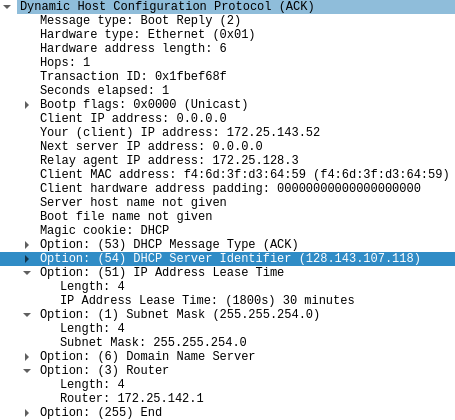
\includegraphics[width=0.55\mypaperwidth]{../arp/dhcp-response3-wireshark.png}
};
%\path[overlay,draw,help lines] (0, 0) grid (15, -8);
\begin{visibleenv}<2>
    \draw[hi box] (0.6, -2.1) rectangle (5.7, -2.45);
    \draw[hi box] (0.6, -2.6) rectangle (5.5, -3.0);
    \draw[hi box] (0.4, -4.1) rectangle (7.5, -7.5);
\end{visibleenv}
\begin{visibleenv}<3>
    \draw[hi box] (0.6, -2.1) rectangle (5.7, -2.45);
    \draw[hi box] (0.4, -4.1) rectangle (7.5, -7.5);
    \matrix[fill=white,nodes={minimum height=0.4cm},
        column 1/.style={nodes={text width=4cm}},
        column 2/.style={nodes={text width=3cm}},
    ] (route table) at (15, -2) {
    addresses \& next hop \\
    172.25.142.0/23 \& (direct) \\
    default \& 172.25.142.1 \\
    };
\end{visibleenv}
\end{tikzpicture}
